\documentclass[tikz,border=4pt]{standalone}
\usepackage{ctex}
\usepackage{pgfplots}
\pgfplotsset{compat=1.18}
\begin{document}
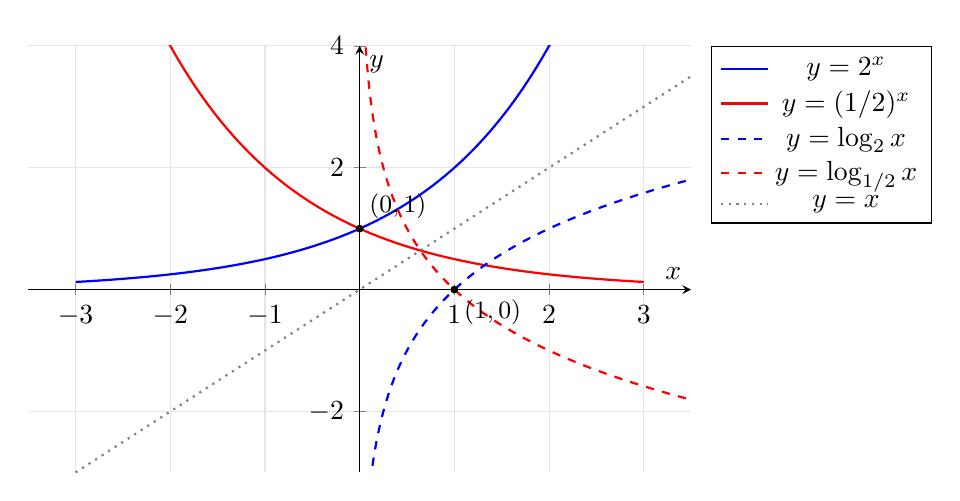
\begin{tikzpicture}
\begin{axis}[
    axis lines=middle, width=10cm, height=7cm,
    xmin=-3.5, xmax=3.5, ymin=-3, ymax=4,
    samples=200, grid=both, grid style={gray!20},
    xlabel={$x$}, ylabel={$y$},
    legend pos=outer north east,
]
\addplot[blue, thick, domain=-3:3] {2^x};
\addlegendentry{$y=2^x$}
\addplot[red, thick, domain=-3:3] {(1/2)^x};
\addlegendentry{$y=(1/2)^x$}
\addplot[blue, dashed, thick, domain=0.001:3.5] {ln(x)/ln(2)};
\addlegendentry{$y=\log_2 x$}
\addplot[red, dashed, thick, domain=0.001:3.5] {ln(x)/ln(1/2)};
\addlegendentry{$y=\log_{1/2} x$}
\addplot[gray, dotted, thick, domain=-3:4] {x};
\addlegendentry{$y=x$}
\node[circle, fill=black, inner sep=1pt] at (0,1) {};
\node[above right] at (0,1) {\small $(0,1)$};
\node[circle, fill=black, inner sep=1pt] at (1,0) {};
\node[below right] at (1,0) {\small $(1,0)$};
\end{axis}
\end{tikzpicture}
\end{document}
